\documentclass[a4paper,12pt]{article}

\usepackage{float}
\usepackage{amsmath}
\usepackage{amsfonts}
\usepackage{amssymb}
\usepackage{graphicx}
\usepackage[margin=0.8in]{geometry}
\usepackage[utf8]{inputenc}

% Title information
\title{Oscillations}
\author{Artur Topal (S5942128), Tyn *******}
\date{11 December 2024}

\begin{document}

\maketitle

\begin{abstract}
This will be our abstract.
\end{abstract}

\section{Introduction}
This is our \textbf{very short} introduction.

\section{Theory}
In a closed damped driven oscillatory system, three forces are acting on a point mass: restoring force ($F_{restoring} = -kx$), damping force ($F_{damping} = -b\dot{x}$), and driving force ($F_{driving} = F_0 \cos(\omega_d t)$). By the Second Newton's law, resulting motion is modelled by:
\begin{equation*}
    m\ddot{x} + b\dot{x} + kx = F_0 \cos(\omega_d t)
\end{equation*}

More commonly, this differential equation is written as
\begin{equation} \label{eq:full_motion}
    \ddot{x} + 2\gamma \dot{x} + \omega^2 x = \frac{F_0}{m} \cos(\omega_d t)
\end{equation} where $\gamma = \frac{b}{2m}$ is the damping factor, $\omega = \sqrt{\frac{k}{m}}$ is natural angular frequency of the oscillations.

% refer to Morin for further information
Depending on the value of $\Omega^2$, there are three cases to consider: \textbf{underdamping}, \textbf{overdamping}, and \textbf{critical damping}. In this experiment, the damping factor was chosen in a way that the oscillatory system is underdamped ($\Omega^2 < 0$). In this case, after long enough time, the inital oscillations will die out, and the system will oscillate with some amplitude $A$ at the driving frequency $\omega_d$ but shifted by some phase $\phi$.
The amplitude can be found to be:
\begin{equation} \label{eq:full_motion_ampl}
  A = \frac{ F_d/m  }{ \sqrt{ (\omega^2 - \omega_d^2)^2 + (2\gamma \omega_d)^2 } }
\end{equation}
The phase is:
\begin{equation} \label{eq:full_motion_phase}
  \tan(\phi) = \frac{2 \gamma \omega_d}{\omega^2 - \omega_d^2}
\end{equation}

There is one frequency when the amplitude from Eq.~\eqref{eq:full_motion_ampl} is maximized. This particular frequency is called \textbf{resonance frequency}, $\omega_{res}$. The behavior of the damped driven oscillatory system at resonance frequency is further addressed in appendix \ref{appendix:preps}.  

In this experiment, the system is modelled using above equations since the restoring force comes from the springs, driven force is harmonic, and the damping force depends on the change of magnetic flux, which in our case depends on the speed. The only difference is that displacements ($x(t)$) and speeds are angular.  


\section{Experimental setup}
The main objective of this experiment was to investigate the oscillatory motion of a damped harmonic oscillator that was driven by an electric motor. The experimental setup depicted in Figure 1 consists of an oscillation disc at the top, that is equipped with a rotation sensor to measure the angular displacement. A magnet that adds a damping term is located next to the disc. An electric motor at the bottom of the set up delivers a driving force, above the motor a second rotary motion sensor is located to measure the frequency and phase of the driving force.
%image of setup

Also, this is \textbf{how you plan to obtain your data and how this will lead to the final result.} 


\section{Results}
\subsection{Direct Calculation of Damping} \label{sec:direct_damping}

The oscillations produced without an added damping factor, i.e. the magnet are displayed in Figure 2. The assumption was made that the string to which the springs were attached did not slip from the pulley. Figure 2 shows underdamped oscillations, which can be seen by a decrease in amplitudes. The oscillations produced without an added damping factor, i.e. the magnet are displayed in \ref{fig:undamped_oscillations}. The assumption was made that the string to which the springs were attached did not slip from the pulley.

\begin{figure}[h!]
  \centering
  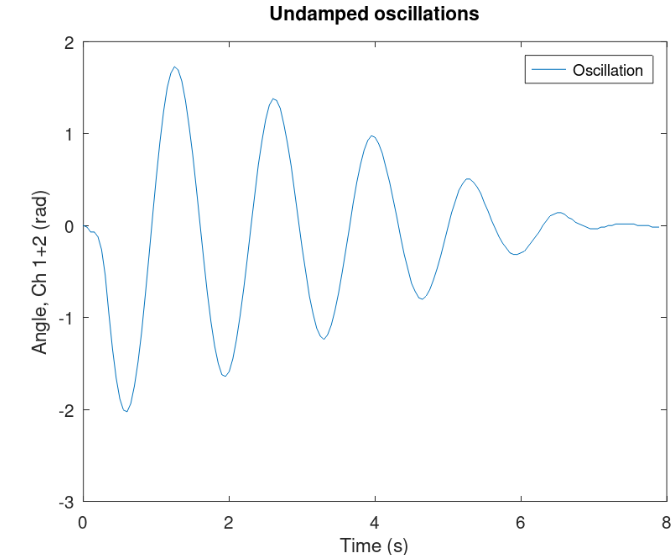
\includegraphics[width=1\textwidth]{oscillations/images/Undamped_Oscillations}
  \caption{Oscillations without damping}
  \label{fig:undamped_oscillations}
\end{figure}

From the measurements the coordinates of the maxima were determined and from this the natural frequency was determined to be $\omega = 4.8 \pm 0.1 (rad/s)$, which was constant throughout the measurements.

A damping term was added by placing the magnet back in its original position, the oscillations are displayed in \ref{fig:underdamped}. The coordinates of nine of the maxima were determined and were plotted in \ref{fig:log of damping factor}. 

\begin{figure}[h!]
  \centering
  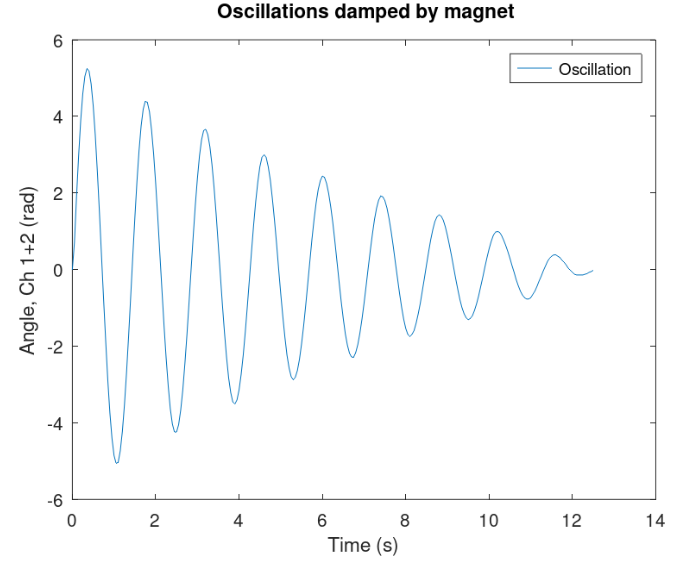
\includegraphics[width=1\textwidth]{oscillations/images/underdamped}
  \caption{Decrease in amplitude by an added damping term}
  \label{fig:underdamped}
\end{figure}

\begin{figure}[h!]
  \centering
  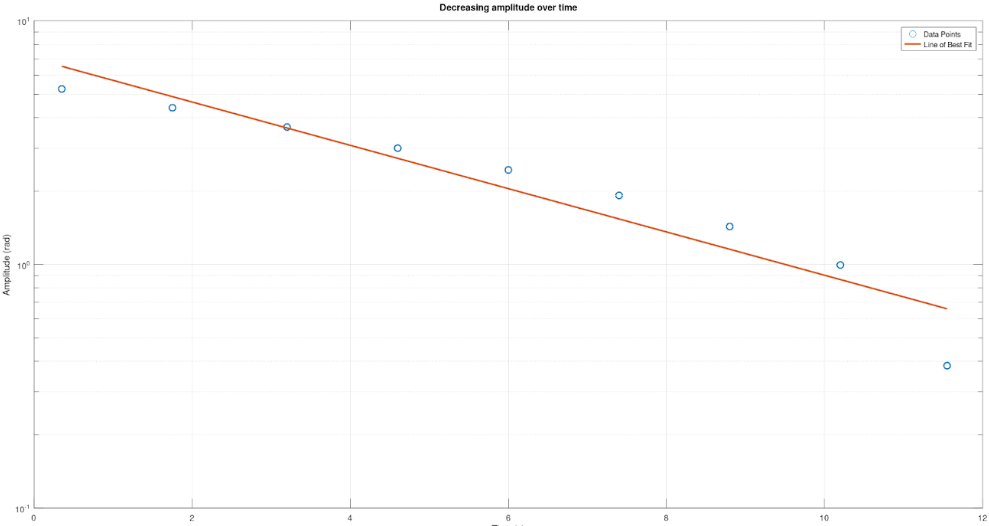
\includegraphics[width=1\textwidth]{oscillations/images/log}
  \caption{Semi-logaritmic plot of the amplitude over time}
  \label{fig:log of damping factor}
\end{figure}

The displacement amplitude $x(t)$ decreases with:
\begin{equation}
  x(t) = e^{-\gamma t} \cos(\omega t + \phi) 
  \label{eq:displacement amplitude}
\end{equation}
The slope of the line of best fit $l$ is equal to the $-\gamma$ term in Equation .
\begin{equation}
  |l| = \gamma 
\end{equation}

By this a damping factor of $\gamma_{direct} = 1.3 \pm 0.2 (rad/s)$ was determined.

\subsection{Indirect Calculation of Damping} \label{sec:indirect_damping}

\begin{figure}[H]
  \centering
  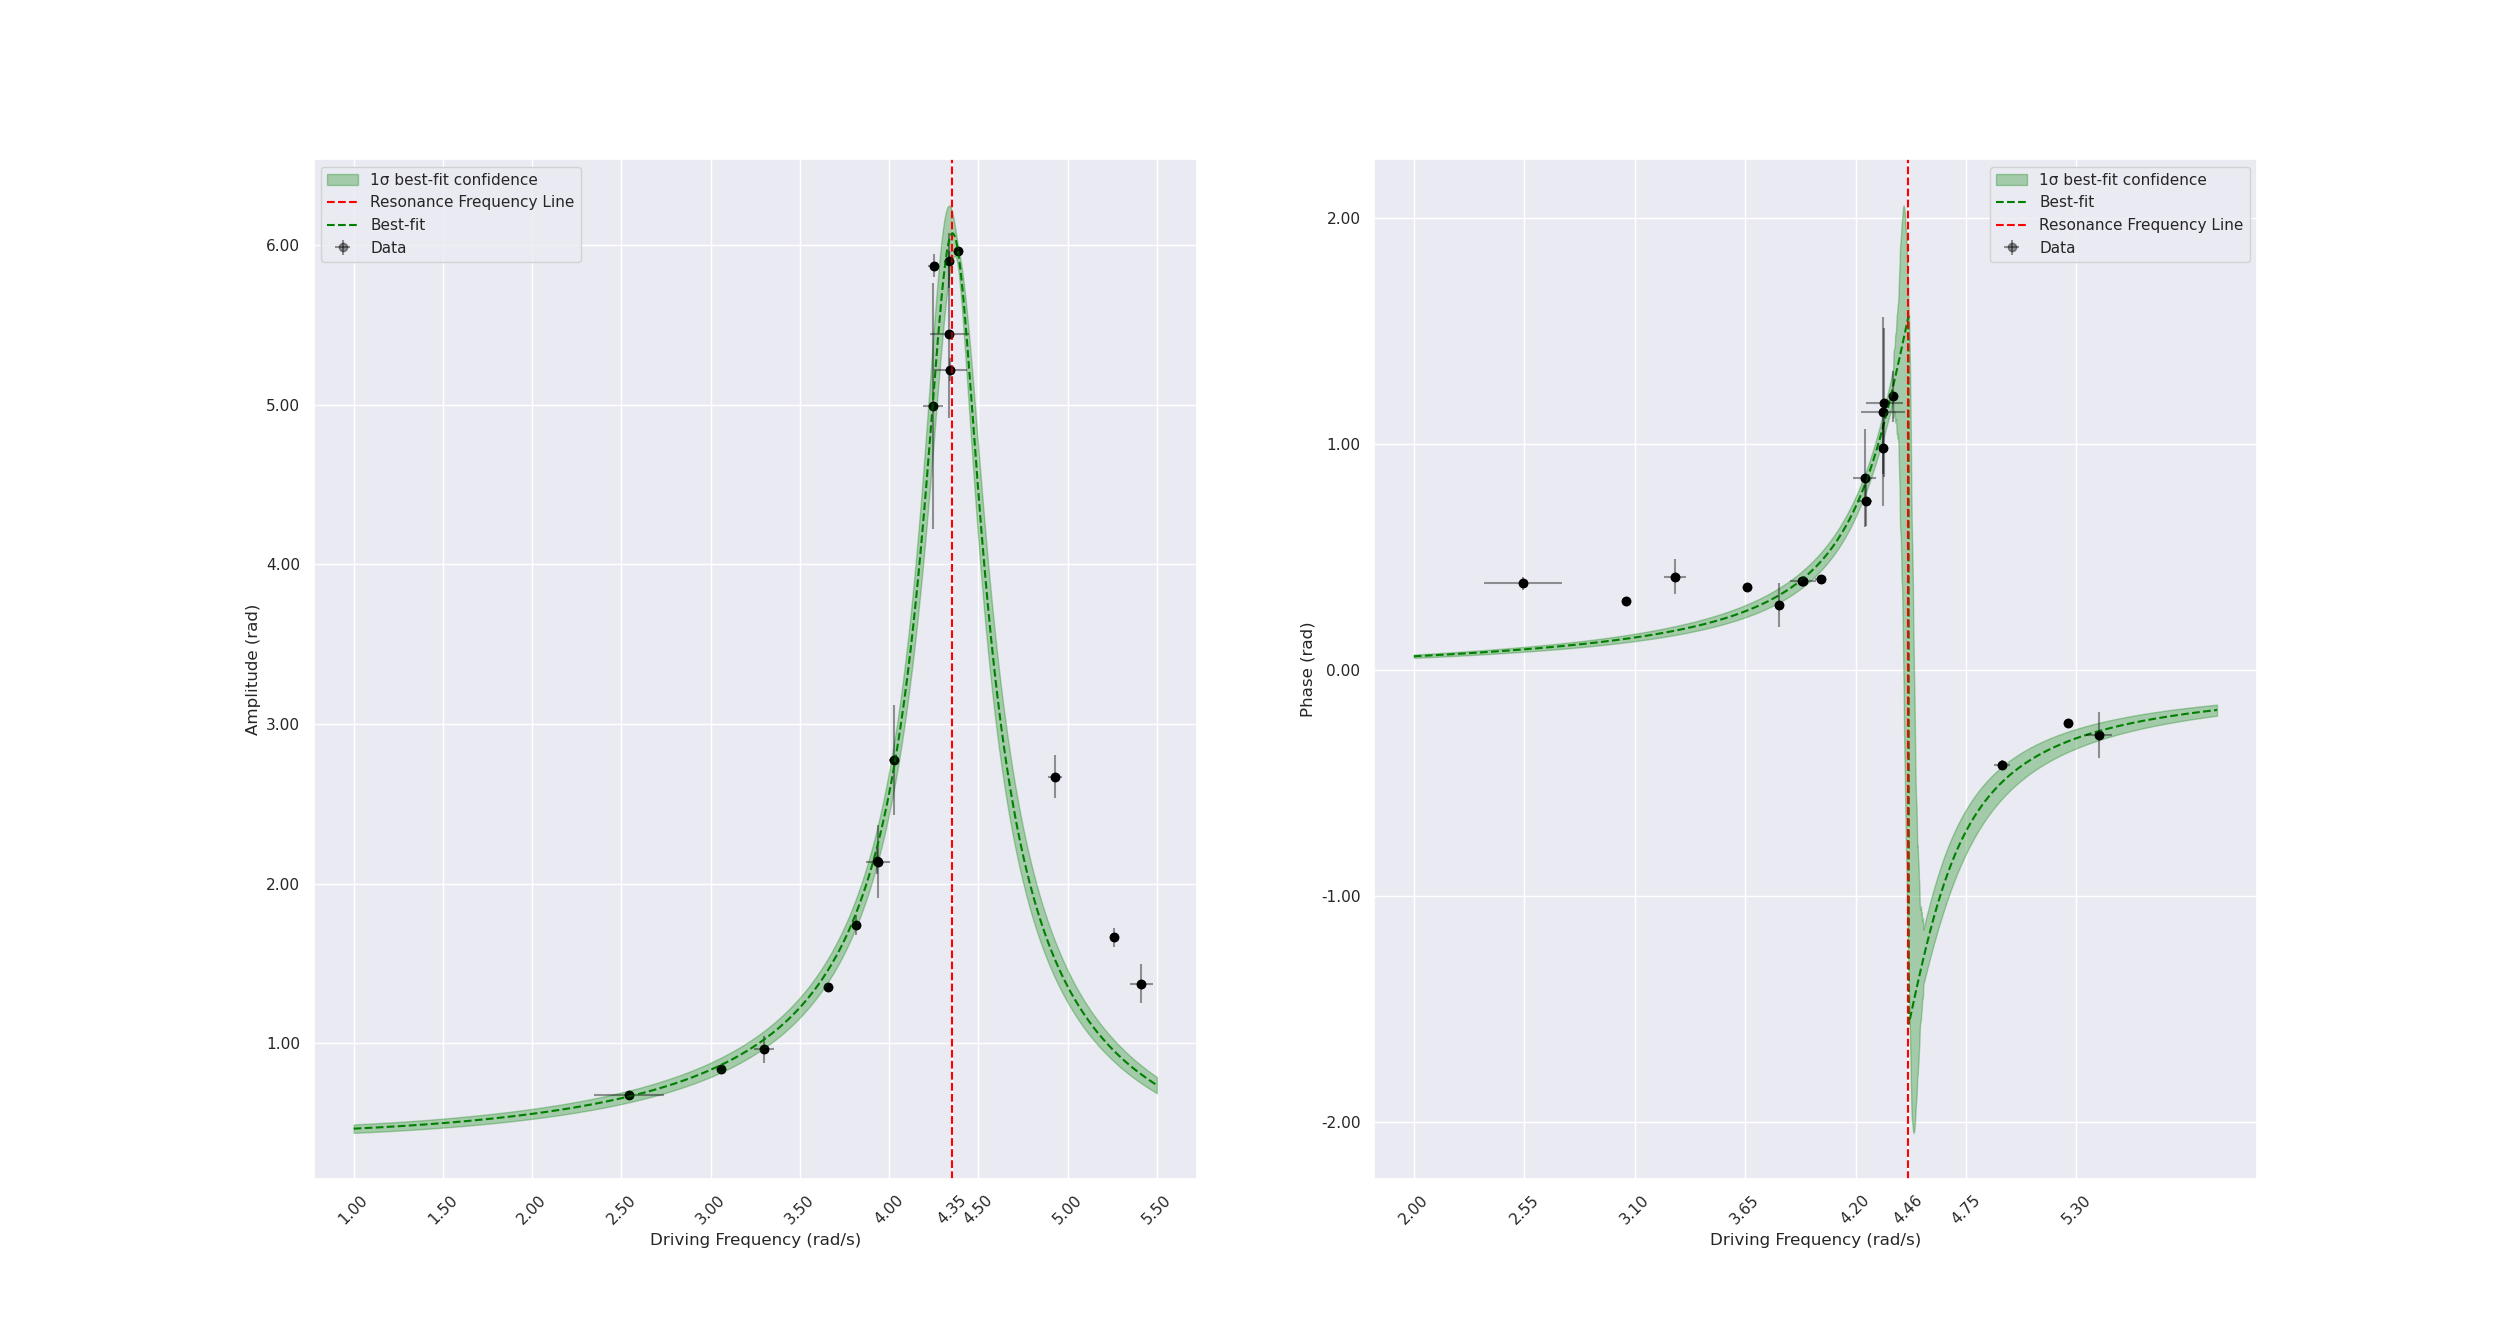
\includegraphics[width=1\textwidth]{oscillations/images/resonance}
  \caption{Amplitude and phase difference of the oscillations plotted against driving frequency.}
  \label{fig:resonance}
\end{figure}

Oscillations of the damped driven system were recorded for different values of the driven force\footnote{There is a linear relation between the driving force and the input voltage.}. The graph of the amplitude and phase difference of the oscillations against driving frequencies with best-fit curves and correspoding uncertanties are depicted in Fig.\ref{fig:resonance}. Tabular data with respective errors are depicted in Table \ref{tab:data}.

Resonance frequency from the amplitude-frequency graph is estimated to be $\omega_{amplitude} = 4.35 \pm 0.09 (rad/s)$. Resonance frequency from the phase-frequency graph is estimated to be $\omega_{phase} = 4.46 \pm 0.02 (rad/s)$. Combined resonance frequency is

\begin{equation*}
\omega_{r} = \frac{\omega_{amplitude} + \omega_{phase}}{2} \pm \sqrt{\sigma(\omega_{amplitude}) + \sigma(\omega_{phase})} = 4.41 \pm 0.09 (rad/s)
\end{equation*}

Damping factor is again evaluated from Eq.~\ref{eq:freq_deps}.

\begin{equation*}
        \gamma_{indirect} = \sqrt{ \frac{\omega^2 - \omega_{res}^2}{2} } = \sqrt{ \frac{4.79^2 - 4.41^2}{2} } = 1.32 \pm 0.8 (rad/s)
\end{equation*}       

This damping factor matches the damping factor previously calculated ($\gamma_{direct}$).

Error analysis for the resonance frequencies and the (indirect) damping factor is located in Appendix \ref{appendix:errors}.


\section{Discussion}
Our discussion of the results of the experiment.


\section{Conclusions}
To conclude, experimentally calculated damping factors, resonance frequency, and natural frequency followed the hypothesis. Future improvements of the setup are the performance of the experiment on a more stable base, usage of rotary sensors with a higher time-resolution and more precise measurements of displacements and derivatives. Slipping of the strings should be minimized by restricting the angular motion of the springs and strings.


\appendix
\section{Appendix A}
\textbf{Exercise 1.} \\
Question: Briefly state the first question here.

\textbf{Answer:} Provide a concise answer to the first question. Include any relevant calculations or explanations if necessary. For example:
\[
F = m \cdot a
\]

\vspace{1em}

\textbf{Exercise 2.} \\
Question: Briefly state the second question here.

\textbf{Answer:} Provide a concise answer to the second question. Include diagrams or references if needed. For example:

\vspace{1em}

\textbf{Exercise 3.} \\
Question: State the third question here.

\textbf{Answer:} Explain the answer briefly. For example:
The energy conservation law can be expressed as:

\[
f_{x} = \frac{a}{b}
\]

where \(K\) is the kinetic energy and \(U\) is the potential energy.



% IMPORTANT
% we may wanna add acknowledgements, references, etc.

\end{document}
